\section{Рассеяние Ми}

В 1908 году немецким физиком Густавом Ми было получено \cite{Mie1908} решение уравнений Максвелла для рассеяния света на сферических частицах произвольного радиуса. В случае когда размер частицы гораздо меньше длины волны рассеиваемого света, рассеяние Ми является частным случаем Рэлеевского рассеяния. Часто под рассеянием Ми подразумевают рассеяние света на частицах с размерами, сравнимыми с длиной волны взаимодействующего света. Распределение электрического поля внутри сферы для первых четырёх мод с комментариями из \cite{Bohren1998} показано на рисунке \ref{fig:mie_example}.

\begin{figure}[H]
	\centering
	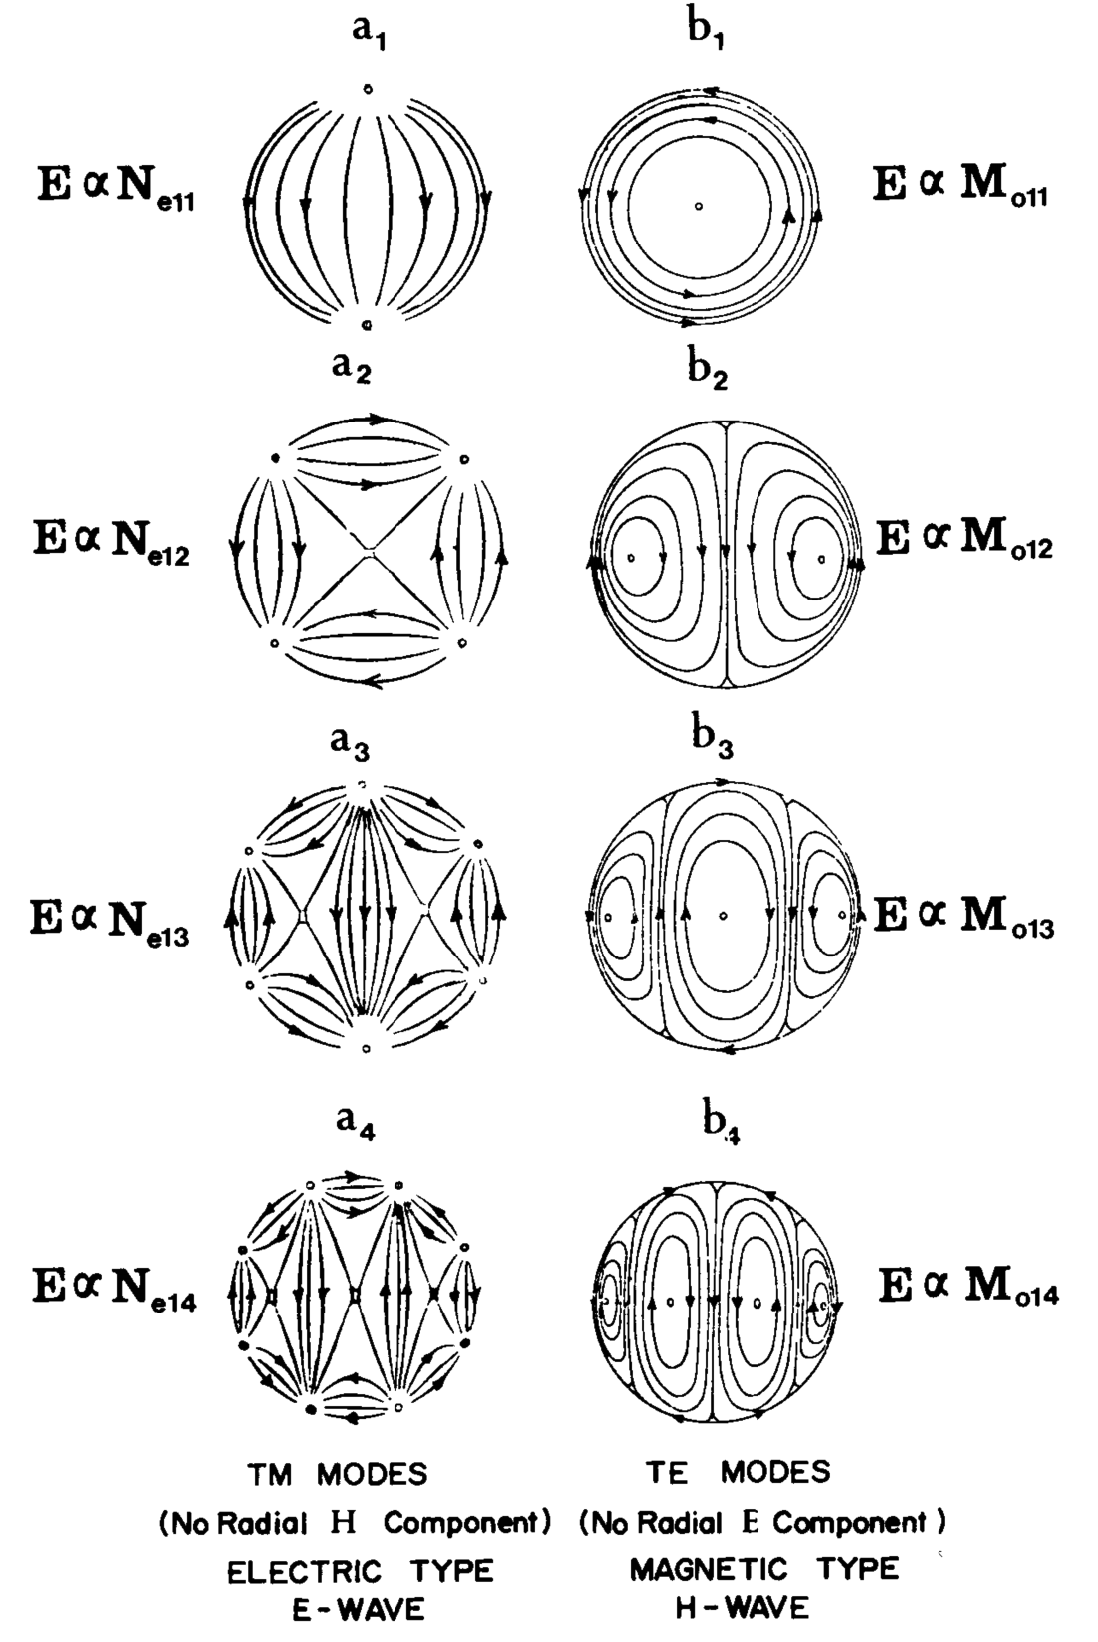
\includegraphics[width=0.75\textwidth]{img/Mie_total}
	\caption{Распределение электрического поля для первых четырёх резонансов Ми}
	\label{fig:mie_example}
\end{figure}

Ми-резонансные наночастицы являются удобным объектом для создания метаматериалов. В 1947 году было предложена \cite{Lewin1947} модель, описывающая композитный материал, состоящий из массива магнитодиэлектрических сфер с $\varepsilon_1, \mu_1$, встроенного в фоновый материал ($\varepsilon_2, \mu_2$). В этом случае теория Ми предсказывает следующие значения эффективных диэлектрической и магнитной проницаемостей $\varepsilon_{eff}$ и $\mu_{eff}$:

\begin{equation}
	\varepsilon_{eff} = \varepsilon_1 \left(1 + \frac{3 v_f}{ \frac{F(\theta) + 2b_e}{F(\theta) - b_e} - v_f } \right)
\end{equation}

\begin{equation}
	\mu_{eff} = \mu_1 \left(1 + \frac{3 v_f}{ \frac{F(\theta) + 2b_m}{F(\theta) - b_m} - v_f } \right)
\end{equation}

где

\begin{equation}
	F(\theta) = \frac{2 \left( \sin \theta - \theta \cos \theta\right)}{\left( \theta^2 - 1 \right) \sin \theta + \theta \cos \theta}
	\label{eq:resonance function}
\end{equation}

\begin{equation}
	b_e = \varepsilon_1 / \varepsilon_2, \quad b_m = \mu_1 / \mu_2
\end{equation}

\begin{equation}
	v_f = \frac{4}{3} \pi \left( \frac{r_0}{p} \right)^3, \quad \theta = k_0 r_0 \sqrt{\varepsilon_2 \mu_2}
\end{equation}

Уравнение \ref{eq:resonance function} показывает что $F(\theta)$ является резонансной функцией и принимает отрицательные значения в некоторой области параметра $\theta$ вблизи резонанса, что приводит к отрицательным значениям $\varepsilon_{eff}$ или $\mu_{eff}$.

В этой модели учитывались лишь первые и вторые резонансные моды, поскольку высшие резонансы Ми часто возникают на частотах, на которых не применима формула Клаузиуса — Моссотти. Позже эти расчёты были улучшены в работе \cite{Jylha2006} путём принятия во внимание электрической поляризуемости сфер, находящихся в режиме магнитного резонанса.

Как уже упоминалось выше, для получения эффективного магнитного резонанса как правило требуется использовать наноструктуры, содержащие металлические элементы \cite{Zhao2009}. Однако присутствие металла неизбежно приводит к омическим потерям, что делает подобные металлсодержащие среды практически невозможными к использованию в полях высотой интенсивности, требуемой для изучения нелинейно-оптических свойств. Из этого ограничения вытекает интерес и необходимость в реализации магнитного резонанса в чисто диэлектрических метаматериалах. Впервые полностью диэлектрические структуры, обладающие оптическим магнетизмом были получены в работе \cite{Ginn2012}. Дополнительным плюсом подобных решений является большая независимость от угла и более удобные возможности для интеграции в трёхмерные структуры.